\documentclass{llncs}
\usepackage{xcolor}
\usepackage{listings}
\setcounter{tocdepth}{5}
\setcounter{secnumdepth}{5}
\usepackage{hyperref}
\usepackage{graphicx}

\hypersetup{
    colorlinks,
    citecolor=black,
    filecolor=black,
    linkcolor=violet,
    urlcolor=black
}

\lstdefinelanguage{Coq}{
  ,morekeywords={match,end,Definition,Inductive,Lemma,Record,
    Variable,Section,case,of,if,then,else,is,let,in,do,return,with}%
  ,keywordstyle=\bfseries
  ,basicstyle=\sffamily
  ,columns=fullflexible
  ,numberstyle=\tiny
  ,escapeinside={@}{@}
  ,literate=
  {<-}{{$\leftarrow\;$}}1
  {=>}{{$\rightarrow\;$}}1
  {->}{{$\rightarrow\;$}}1
  {<->}{{$\leftrightarrow\;$}}1
  {<==}{{$\leq\;$}}1
  {\\/}{{$\vee\;$}}1
  {/\\}{{$\land\;$}}1
}

\lstset{language=Coq,breaklines=true,basicstyle=\footnotesize}%%, frame=single}
\usepackage{scrextend}

\begin{document}

\title{Graphics in Coq for use in ...}
\author{Nathan St. Amour \and ...}
\institute{Ohio University, Athens, OH 45701}
\maketitle

\begin{abstract}
We present a method for modeling graphics in coq that provides an intuitive way to certify and generate graphical programs by using the interactive
theorem prover Coq.  Our implementation uses a set of graphics primitives that can be used to implement typical functions that a user would expect in a *nix like standard library for graphics.  We show proof of concept and ease of extraction from the Coq code to OCaml. 
\end{abstract}
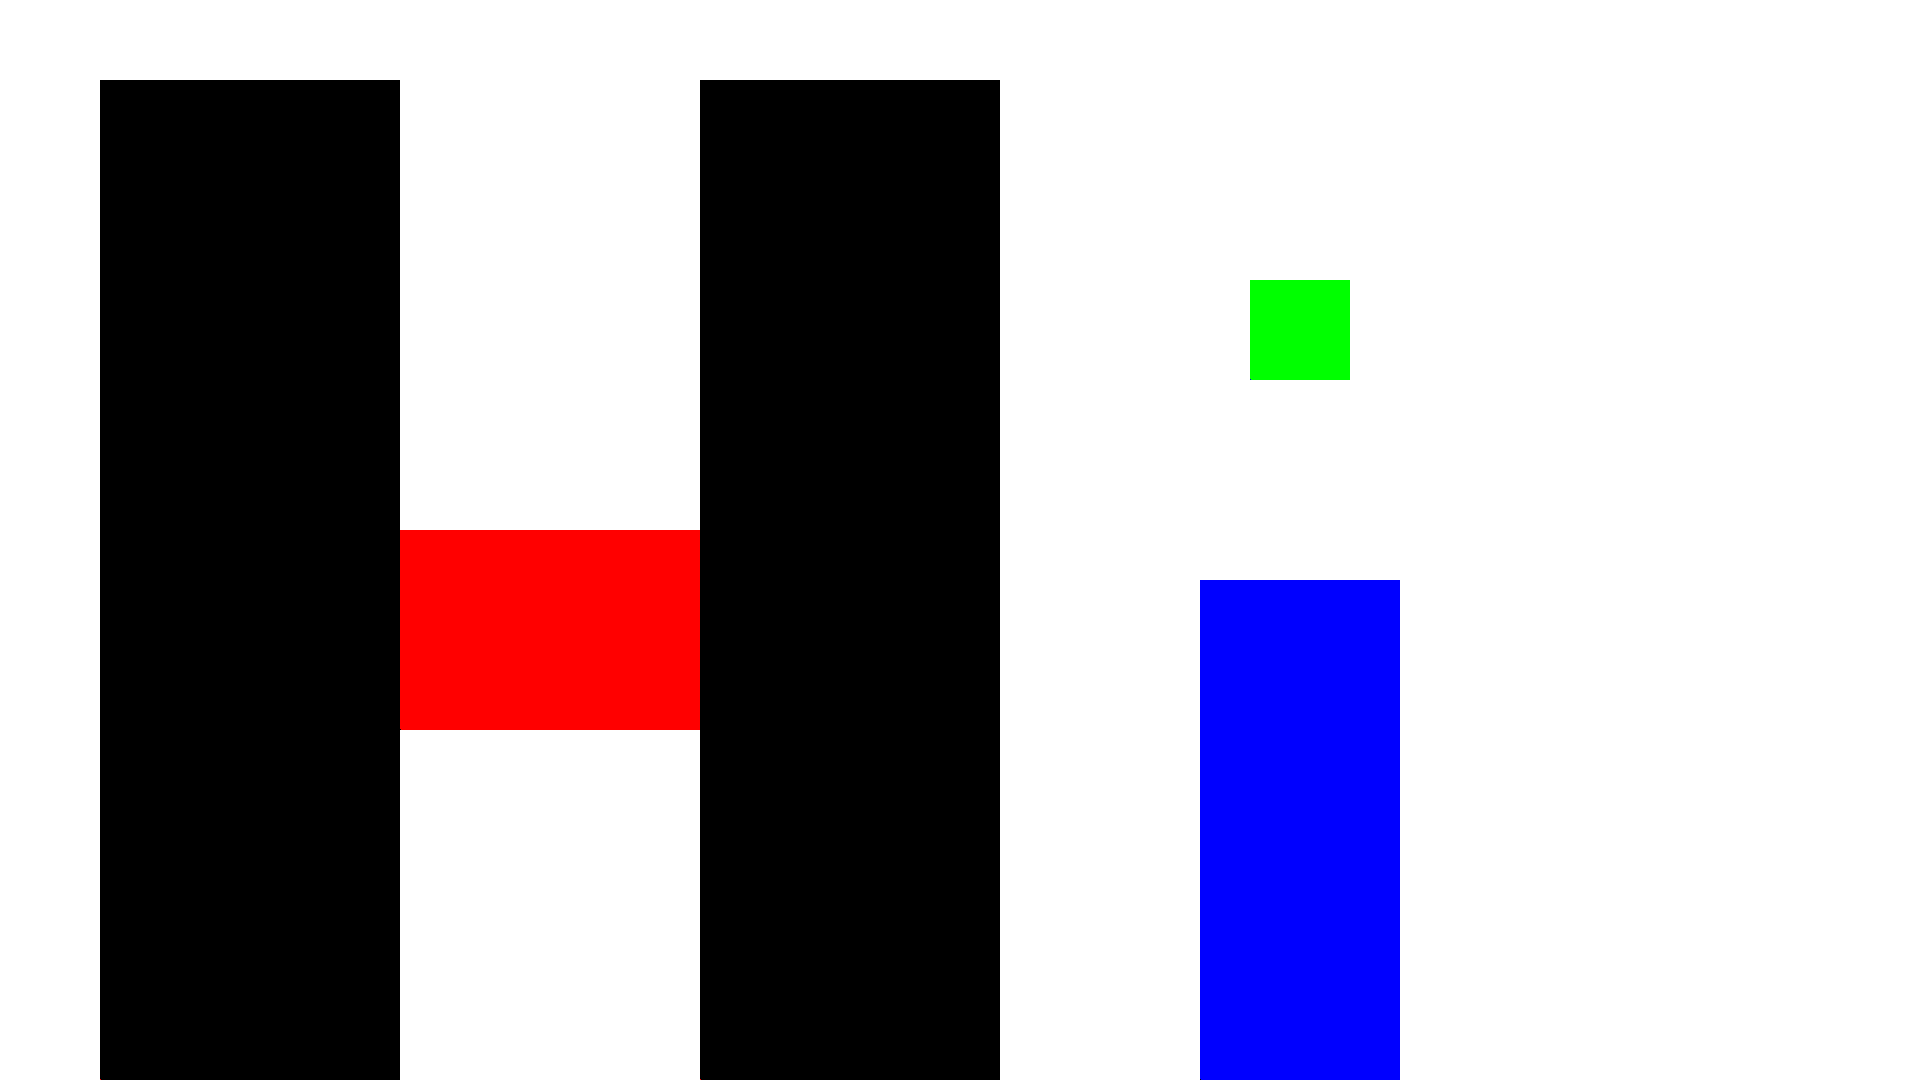
\includegraphics[scale=.3]{hi.png}

\tableofcontents
\newpage

\section{Introduction}

Creating graphical programs may not be the first thing on the minds of the bold people using a purely functional proof assistant such as Coq.
You should be easily convinced that this is the case by the resounding lack of any attempt at modeling graphics in Coq.  However there are people
who have put work into the formalization of geometry in Coq. There are two components of our implementation that provide it with flexibility and congruence between any instance. There is a type class that lives at the highest level of our implementation.  The primary function of the type class is to provide functions that use the graphics primitives to affect a state that must be given when providing an instance of the type class. The next key component is the ability to be flexible with an instance of this graphics type class.  We have been able to write two instances that hold as a proof of concept for the graphics implementation.  The first instance uses finite maps to store the state of what has been drawn to the screen.  We have been successful in proving properties about the correctness of drawing lines, particularly in the vertical and horizontal directions, and regular rectangles drawn with lines that are either vertical or horizontal.  The corresponding functions for filling rectangles has also been proven.  The other instance of the graphics class is an axiomatic way of implementing the graphics in OCaml.  This is achieved by exporting the draw\_pixel command to the OCaml graphics plot command which is then called by the interp function in our graphics type class to draw to the screen.
The with some work the graphics implementation that we present could become a rhobust tool for developing graphical programs.

\section{Similar Projects}
During our external research, we could not find another project where someone
implemented a graphics library inside of Coq, however, there are many other
functional languages that implement a graphics library. Examples of others
are: Haskell, Scheme, Ocaml and pretty much any other functional language in
which we can use axioms to instantiate the graphics primitives. The functional
language that we focused on for our implementation of a graphics library was
Ocaml graphics library. We chose to use the Ocaml graphics library as the
model for our Coq graphics library for a few reasons. The most important
aspect of Ocaml that led to use using it over any other functional language is
that Coq is written in Ocaml, which makes translating and exporting functions
from Ocaml to Coq more intuitive than if we had used another language like
Haskell or Scheme. We took functions from the Ocaml graphics library like plot,
open\_graph, color, lineto and implemented equivalent functions in Coq and
then exported them as Ocaml to be displayed. In addition to recreating some
of the Ocaml graphics functions in Coq, we also implemented some supporting
functions like draw\_rect and fill\_rect and we proved some theorems about the
specifications of these functions.

Even though there have not been any attempts to implement a graphics library
in coq, there has been research done in the verification of the specifications of
geometric shapes in Coq. In Pham and Bertot’s paper “A Combination of a 
Dynamic Geometry Software With a Proof Assistant for Interactive Formal Proofs,”
\cite{geo} they adapted Coq’s tactic language to allow users to interactively
construct simple proofs about geometric shapes.



\section{Stucture Of code}

\subsection{The Graphics Type Class}
 To begin we have implemented the syntax of a language of graphics commands(g\_com). The semantics of this language are defined in an interesting way, leaving the type of what we will call the current state of the screen as the type Type.  By not specifying the type of the state we are able to
 provide a single implementation of functions that only rely on a small set of primitives that can be changed to reflect a certain goal. We are then able to define an instance of the class by meeting the requirments outlined. We currenlty have instantiated two instances of the graphics\_prims type class. \cite{class}

\begin{lstlisting}
   Inductive g_com : Type :=
    | draw_pix : point -> color -> g_com
    | open_graph : point -> g_com
    | resize_window : point  -> g_com
    | lineto : point -> point -> color -> g_com
    (* | draw_circle : point -> Z -> g_com *)

   (* Rec with the bottom left point followed by the top right.*)          
    | draw_rect : point -> point -> color -> g_com
    | fill_rect : point -> point -> color -> g_com
    | seq : g_com -> g_com -> g_com.

   Notation "a ;; b" := (seq a b) (at level 50, left associativity).

   (*These are the basic primitives that we build everything from*)
   Class graphics_prims (T :Type) :=
   mkGraphicsPrims
   {
     init_state : unit -> T;
     update_state : T -> point -> T;

     (*Add an update color*)
     draw_pixel : T -> point -> color -> T;

   }.

   Section interp.

    Context {T : Type} `{graphics_prims T}.
  \end{lstlisting}

\subsection{Instances}
We have two instances of the graphics\_prims type class.  One that uses a map over pairs of integers(points) : $point -> color$ and another that
uses axioms to allow for extraction into OCaml.

  \subsubsection{OCaml}
  \subsubsection{Coq State Map}



  



\subsection{Functions for Drawing}
The following functions are what is used to implement an interpretation of the graphics class in a way that does not depend on the implementation than the type.

 \begin{lstlisting}
    Fixpoint interpolate (t : T) (i : nat) (p1 p2 V: point) (num_points : Z) c : T :=
    match i with
     | O => draw_pixel t p1 c
     | 1%nat => draw_pixel t p1 c
     | S i' => let p1' :=
     (((fst p1) + (fst V) * (Z.of_nat i) / num_points),
     ((snd p1) + (snd V) * (Z.of_nat i) / num_points))
     in
     draw_pixel (interpolate t i' p1 p2 V num_points c) p1' c 
    end.

    Fixpoint draw_vline (t : T) (p : point) (c : color) (h : nat) : T :=
    match h,p with
     | O, _ => t
     | S h', (x,y) => draw_pixel (draw_vline t p c h') (x,y+(Z.of_nat h')) c
    end.

    Fixpoint draw_hline (t : T) (p : point) (c : color) (w : nat) : T :=
    match w,p with
     | O, _ => t
     | S w', (x,y) => draw_pixel (draw_hline t p c w') (x+(Z.of_nat w'),y) c
    end.

    Definition interp_draw_line (t : T) (c : color) (p1 p2 : point) : T :=
    interpolate t (Z.to_nat (distance p1 p2) - 1) p1 p2 ((fst p2) - (fst p1), (snd p2) - (snd p1) ) (distance p1 p2) c.

    Fixpoint interp (t : T) (e : g_com) : T :=
     match e with
      | draw_pix p c => draw_pixel t p c
      | open_graph s_size => update_state t s_size
      | resize_window s_size => update_state t s_size 
      | lineto p1 p2 c => let st := interp_draw_line t c p1 p2 in 
       let st' := draw_pixel st p1 c in  draw_pixel st' p2 c
      | draw_rect (x,y) (w,h) c =>
        let w' := Z.to_nat w in
        let h' := Z.to_nat h in
        let t1 := draw_hline t (x,y) c w' in
        let t2 := draw_hline t1 (x,y+h) c w' in
        let t3 := draw_vline t2 (x,y) c h' in
                  draw_vline t3 (x+w,y) c h'
      | fill_rect p (w,h) c => fill_rect_rc t p (Z.to_nat w) (Z.to_nat h) c
      | seq g1 g2 => let st := (interp t g1) in (interp st g2)
     end.

    Definition run (e : g_com) : T :=
    interp (init_state tt) e.
   End interp.
 \end{lstlisting}
 
 
 The draw\_hline and draw\_vline functions are recursive functions that draw horizontal or vertical lines recursively starting at a point with a size n.
 
 The draw\_rect function draws the border of a rectangle starting a point and uses draw\_hline and draw\_vline to draw the sides
 
 fill\_rect recursively creates h horizontal lines of witdth w recursively using the draw\_hline
 
 
% \subsection{Subsection2} This is a second subsection.



% This is a citation.~\cite{gennaro2010non}
% This is a chunk of code:

% \begin{lstlisting}

%   Definition f(x : nat) := S x.

%   Definition g(y : nat) := f y.

% \end{lstlisting}



% This is inline code \lstinline|Fixpoint f(x : nat) := ...| typeset within a line of text.

% \paragraph{Para1.} This is a paragraph, or subsubsection.





\section{Proofs}
To prove the correctness of our drawing functions, we first made a specification of whether a point is in a shape, then we proved that if we draw a shape to a state, then, for any point, if that point is in the shape, the color at that point would be equal to the color of the shape we drew, otherwise the color at that point would be the same as the color in the original state.

The specification for if a point is in a vertical line is as followed

\begin {definition} [on\_vline]
$\forall (x1,y1) \in Z, (x1,y1) \in vline (x2,y2,h) \iff x1 = x2 \land y1 >= y2 \land y1 < y2 + h$
\end {definition}

Our proof of correctness of the drawing a vertical line is as followed

\begin {theorem} [vline\_correct]
$\forall (x1,y1,x2,y2,h) \in Z, \forall c \in Color,\forall st \in State, (x1,y1) \in vline (x2,y2,h) \rightarrow ($ draw\_vline st x2 y2 c $)_{(x1,y2)} = c \land \neg ((x1,y2) \in vline (x2,y2,h)) \rightarrow ($draw\_vline st x2 y2 h c$)_{(x1,y2)} = st_{(x1,y2)} $
\end {theorem}

For this proof we used a lemma that stated that if a point is on a vertical line with height (n+1), then the point is either on the line with height n, or it is equal to the point at the end of the line, or more formally,

\begin {lemma} [vline\_correct\_aux]
$\forall (x1,y1,x2,y1,h) \in Z, (x1,y1) \in $(vline x2 y2 (h+1))$ \iff (x1,y1) \in $(vline x2 y1 h)$ \lor (x1,y1)=(x2,y2+h)$
\end {lemma}


The specification for if a point is in a horizontal line is as followed

\begin {definition} [on\_hline]
$\forall (x1,y1) \in Z, (x1,y1) \in hline (x2,y2,w) \iff y1 = y2 \land x1 >= x2 \land x1 < x2 + w$
\end {definition}

The proof for correctness of draw\_vline was nearly identical to the proof for draw\_hline.
\begin {theorem} [hline\_correct]
$\forall (x1,y1,x2,y2,w) \in Z, \forall c \in Color,\forall st \in State, (x1,y1) \in hline (x2,y2,w) \rightarrow ($ draw\_hline st x2 y2 c $)_{(x1,y2)} = c \land \neg ((x1,y2) \in vline (x2,y2,w)) \rightarrow ($draw\_hline st x2 y2 h c$)_{(x1,y2)} = st_{(x1,y2)} $
\end {theorem}



\begin {definition}[in\_rectangle]
	$\forall (x1,y1,x2,y1,w,h) \in Z, (x1,y1) \in ($rectangle x2 y2 w h$) \iff x1 >= x2 \land y1>=y2 \land x1 < x2 + w \land y1 < y2 + h $
\end {definition}

\begin {theorem} [fill\_rect\_correct]
$\forall (x1,y1,x2,y1,w,h) \in Z, \forall st \in State, \forall c \in Color, (x1,y1) \in $(rectangle x2 y2 w h)$ \rightarrow ($fill\_rect st (x2,y2) w h c$)_{(x1,y1)} = c \land \neg $(rectangle x2 y2 w h)$ \rightarrow ($fill\_rect st (x2,y2) w h c$)_{(x1,y1)} = st_{(x1,y1)}$
\end {theorem}

To prove this, we used the lemma:

\begin {lemma} [fill\_rect\_correct\_aux]
$\forall (x1,y1,x2,y2,w,h) \in Z, (x1,y1) \in ($rectangle x2 y2 w h$) \iff (x1,y2) \in ($hline x1 y2 w$) \land (x2,y1) \in ($vline x1 y2 h$) $
\end {lemma}

This lemma let us replace our definition of in rectangle with the definition of in vline and in hline so we could use our previous lemmas in our proof.


%\section{Maybe stuff to add}
Maybe geometry stuff ? 

There is an educational thing in papers that tried to use coq to make a verified way to prove simple geometric things for students.

Structure of Code

Flattery

Explanation of each function/the type class

Flattery

draw\_vline

Draw\_hline

Draw\_rect

fill\_rect

lineTo

Also add stuff about the specific instances like how they are implemented

Proofs

Pics n’ Shit 

Future plans for project

User Coq to cure cancer 

Conclusions

Flattery




\section{Future Plans}
There have been several plans for addition and improvement that we plan to work on in the future.  Overall the project has been a success for the
time given.  The results of extracting an instance designed for OCaml showed us that implementing functions that draw to a significant fraction of the screen are much too slow for any kind of practical usage.  Since the only primitive that we can use to draw to the screen is draw\_pixel it seems to be impossible to improve the drawing speed.

A possible solution would be a move away from the type class of graphic primitives and into a module.  The idea would be very similar a function for drawing pixels would be provided and all of the previous functions could be implemented as a functor from our new module type for graphics to functions and proofs using the given functions.  However we would then assume for extraction that there is a function that instantly draw all of the points that need to be drawn to the screen.  This would ultimately be a function, $f :Type \rightarrow point \rightarrow point \rightarrow Type,$ with the purpose of either putting all of the points into the map at once, allowing the modeling of what is hopefully something close to the OCaml draw line function and efficient extracted code.

There are multiple properties that could be provided to the module that ensure any instance of the module type would behave in a similar way.  For example the state would have certain properties that it the module type would require.  This is important for writing more general proofs over instances with type for the state and for ensuring that different instances do not implement the new functions in ways that could be incorrect.

It shouldn't be hard to see the merits in writing proofs that live at a level above the implementation.  One of the first proofs that we wrote for the Coq implementation, specifically using maps of type : $point \rightarrow color$, was reasonable to complete at a similar level.  We simply stated the theorem as:
\begin{theorem}
  $\forall$ (t : Type), The two states( st1 st2 : t) that result from drawing two points are the same only if the points are not equal $\land$ the same color is used for pixels drawn that result in the two states.
\end{theorem}

Currently this has been proved by an invariant added to the draw\_pixel function that states this theorem and must be satisfied in order to create an instance of the class.  By using modules and specifications how a state is defined it should be possible to produce a canonical form of any program implemented with draw\_pixel.  From there it shouldn't be hard to provide a reasonable definition of equality between two states, leading to this proofs of this theorem and many others over states.

\begin{lstlisting}
Theorem draw_pixEqualStates : forall (t : T) (p1 p2 : point) (c1 c2 : color),
 p1 <> p2 -> 
   eq (interp t (draw_pix p1 c1 ;; draw_pix p2 c2))
      (interp t (draw_pix p2 c2 ;; draw_pix p1 c1)).
\end{lstlisting}

This provides a proof of concept that using requiring specifications about functions could allow for proofs for any that fits the specifications.
By extending this to the module system in Coq these specifications could be used to build machinery that would prove useful in more advanced generalizations.  The more general proofs would also provide an intuitive way to apply those proofs to additions to instances of the module.

This provides a proof of concept that using requiring specifications about functions could allow for proofs for any that fits the specifications.
By extending this to the module system in Coq these specifications could be used to build machinery that would prove useful in more advanced generalizations.  The more general proofs would also provide an intuitive way to apply those proofs to additions to instances of the module.

We also plan to implement drawing more shapes. We have plans for drawing and filling circles, triangles and arbitrary polygons. We have not included those as the complexity of drawing and writing and proving specifications would be outside of the scope of this project.

Another feature we plan to add is buffers. Our drawing functions could have the ability to draw to a buffer rather than directly to the screen. This buffer could then be drawn to the screen or another buffer. We will add the ability to preform transformations to this buffer, such as translating, rotating, and scaling. Since these are all basic matrix operations, they should be relatively simple to implement.

The last feature we plan to implement is user input. Although coq does not support user-input, we could model the properties of user input in coq, and then leave the implementation to when we export to Ocaml. This would allow us to model an full graphical user interface in coq, which could be used to create simple applications or games.

\section{Conclusion}
In this paper, we outline the creation of our implementation of a graphics
library in Coq. In this project, we were able to implement all the parts that we
expected to, but there is still a lot more work that we can do. We are planning
on adding more functionality to the project and improve some of the existing
implementation. One improvements that we plan to address is the significant
amount of time it takes to fill a shape. An example of a future goal would be
designing more generalized proofs that do not depend on specific implementation
details. An example of this would be, a conical for what has been drawn to the
screen and an equality between two states. This project has been a joy to work
on.


\bibliographystyle{plain}

\bibliography{references}




\end{document}

